\documentclass[letterpaper,twocolumn,12pt]{article}
\usepackage{usenix-2020-09}

% to be able to draw some self-contained figs
\usepackage{tikz}
\usepackage{amsmath}
\usepackage{hyperref}

% % inlined bib file
% \usepackage{filecontents}

% %-------------------------------------------------------------------------------
% \begin{filecontents}{\jobname.bib}
% %-------------------------------------------------------------------------------
% @Book{arpachiDusseau18:osbook,
%   author =       {Arpaci-Dusseau, Remzi H. and Arpaci-Dusseau Andrea C.},
%   title =        {Operating Systems: Three Easy Pieces},
%   publisher =    {Arpaci-Dusseau Books, LLC},
%   year =         2015,
%   edition =      {1.00},
%   note =         {\url{http://pages.cs.wisc.edu/~remzi/OSTEP/}}
% }
% @InProceedings{waldspurger02,
%   author =       {Waldspurger, Carl A.},
%   title =        {Memory resource management in {VMware ESX} Server},
%   booktitle =    {USENIX Symposium on Operating System Design and
%                   Implementation (OSDI)},
%   year =         2002,
%   pages =        {181--194},
%   note =         {\url{https://www.usenix.org/legacy/event/osdi02/tech/waldspurger/waldspurger.pdf}}}
% \end{filecontents}

%-------------------------------------------------------------------------------
\begin{document}
%-------------------------------------------------------------------------------

%don't want date printed
\date{}

% make title bold and 14 pt font (Latex default is non-bold, 16 pt)
\title{\Large \bf Towards CANLay: In-Vehicle Data Transportation for Long}

% %for single author (just remove % characters)
% \author{
% {\rm Jacob Jepson}\\
% Colorado State University
% \and
% {\rm Subhojeet Mukherjee}\\
% Colorado State University
% % copy the following lines to add more authors
% \and
% {\rm Jeremy Daily}\\
% Colorado State University
% } % end author

\maketitle

%-------------------------------------------------------------------------------
\begin{abstract}
%-------------------------------------------------------------------------------
Your abstract text goes here. Just a few facts. Whet our appetites.
Not more than 200 words, if possible, and preferably closer to 150.
\end{abstract}

\section{Introduction and Background}
%-------------------------------------------------------------------------------
In recent years security of the Controller Area Network (CAN) has been a much talked about topic of research. CAN is a broadcast media that enables reliable and low-latency communication between in-vehicle devices, also referred to as Electronic Control Units (ECU). This broadcast nature of CAN, along with the fact that it is inherrently unauthenticaed, makes it susseptible to network-wide cyber threats. 
It has been shown \cite{checkoway_comprehensive_2011, mukherjee_practical_2016,burakova_truck_2016} that remote interfaces on modern vehicles can be used to intrude into CAN networks and inject message to control and/or disrtupt the operations of the vehicle.
% MHD vehicles expose similar interfaces that can be used to control/disrupt critical functions \cite{mukherjee_practical_2016,burakova_truck_2016} typically operated by ECUs using sensors and actuators. 
% In general, security reseach in this area 
To evaluate the effectiveness of their approaches, researchers have typically experimented on real-vehicles or homegrown testbed setups that mimic real vehicles. 
While most households in the United States have at least one passenger car\footnote{\url{https://www.statista.com/statistics/551403/number-of-vehicles-per-household-in-the-united-states/}}, this is not the same for medium and heavy-duty (MHD) vehicles. 
Moreover, creating homegrown testbeds is both logistically and economically challenging. To that end, the need for a publicly accessible testbench is imminent. This is where the concept of the Software Define Truck (SDT) \cite{mukherjee_towards_2021} is critical to the in-vehicle networking community. It aims to provide a distributed virtualization infrastructure on which in-vehicle security experiments can be performed. Although proposed primarily for the heavy-trucks, SDT can easily be adapted for light-weight passenger vehicles as well. SDT's information exchange goal is shown in figure \ref{fig:goal}. CAN frames and physical signals need to be exchanged between ECUs and vehicle simulators located in different subnetworks accross the globe. CANLay is the designed to be the networking backbone of SDT and provide the neccesseary infrastructure to enable this service.

\begin{figure}[t!]
    \centering
    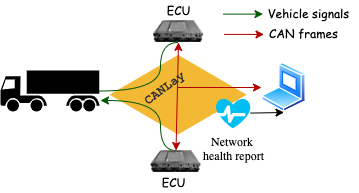
\includegraphics[width=\linewidth]{images/design_goal.drawio.png}
    \caption{Scope of CANLay}
    \label{fig:goal}
\end{figure}

Previous research \cite{tagarev_automotive_2021} has established two critical quality evaluation criteria for testbeds namely, fidelity and adaptability. Fidelity is the ability to emulate a real-world in-vehicle networking infrastructure to the best. Adaptability is the ability to emulate different real-world in-vehicle networking infrastructures. As such, it may be difficult to optimize both these criteria at the same time. To make a system adaptable, the underlying components need to be virtualized so they can be reconfigured to suit user needs. Albeit, this hampers the fidelity of the system. While CANLay allows on-demand network configuring, it also provides a real-time health report for the underlying network. This allows the user to assess the fidelity of the overlay in terms of standard networking metrics like latency, rate of packet drop, etc.

Network virtualization for CAN has been approached in different ways. First, there has been the software-defined-networking adapted for CAN. This approach is largely hardware basd and is targetted primarily for in-vehicle networking, not over long range networking. For range relaying of CAN frames, there has been the CAN-to-ethernet direction of research. Reconfigurability and network performance has not been a cornerstone for these systems. Then again, neither of these paradigms have been designed to transport vehicle signals over long distances. A few research works have ventured into that area. Albeit, they have not resorted to network virtualization for the same.

In the rest of this paper.

% \section{Related Work}
% A recent survey presents a broad overview. 
% THe main concerns are fidelity and adaptbility. More you virtualize, more you loose fidelity. 
% There is no general about to an optimum measure but it depends on the type of experimentation the testbed aims to support. Experiments could be reliant on subtle physical features or the data being transmitted. Virtualization is suited for the first kind, while definitely providing greater adaptbility. Virtualization can be applied at three levels namely, ECUs, network, and physical. 
% ECU virtualization may be critical but extremely challenging to acheive due to intellectual property regulations. 
% Network virtualization may be a more viable route but, to the best of our knowledge, most testbed proposals have eluded this feature. Albeit, experiments that rely on low-level features of networking, like signaling schemes and timing patterns may be difficult to acompolish here, but it may be a more concrete ground for data oriented reseach with certainly a more diverse specturm of testing setups. 


% \section{Design Goals}
% \begin{figure}[t!]
%     \centering
%     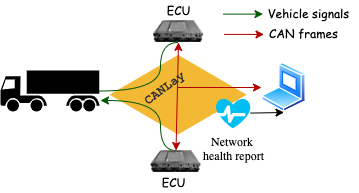
\includegraphics[width=\linewidth]{images/design_goal.drawio.png}
%     \caption{Design Goal of CANLay}
%     \label{fig:goal}
% \end{figure}
% The overarching design goal of this project is elucidated through figure \ref{fig:goal}. Routing physical signals and CAN frames between ECUs, a vehicle simulator of some sort that can produce and consume the signals, and a laptop that can act as the user's gateway to this communication portal. In phase 1 our goal was to enable digital networking between these endpoints and focus on the analog parts at a later phase. Mentioned below is a list of tasks we aimed to accomplish in phase 1. 
% \begin{itemize}
%     \item A means to communicate simulator generated signals to ECUs. We decided to generate the structural and behavioral aspects  the networking framework first 
% \end{itemize}

% To design a platform that simulates a CAN internetwork within a running vehicle using ECUs from separate subnets within the internet a. la. the software-defined truck \cite{mukherjee_towards_2021}. 
% Clearly, this has to be achieved over in-vehicle communication overlays on top of protocols of the internet.

% The distributed overlay nature of the project introduces a set of fidelity-related challenges when emulating the tightly integrated infrastructure within the vehicle. 
% Firstly, CAN provides a low-latency, strong reliability communication media that may be difficult to emulate over long-range communication channels. This requirement is even stronger for the physical signals that are usually transmitted over direct wiring in a real-world setting. 
% % A major requirement of this project is, therefore, to provide adequate assurance about the quality of communication in the overlay network. 
% Secondly, the broadcast nature of CAN may be difficult to realize in a distributed manner over the (typically) unicast internet protocols. Using unicast packets for multi/broadcast may require duplication in linear time. This is both space and time-intensive, especially if performed in a smaller scale local network that has limited bandwidth.
% The final challenge is to realize the complexity of interactions between the different components of the vehicle that normally operate in the same physical setting.
%TODO Dr. Daily, provide an example here

% Albeit, all of these challenges can be difficult to realize in full in an adaptability-centric setting like ours. Even so, a major goal of this project is to optimize and report the quality of experimentation, thereby creating a transparent and usable environment for the experimenter. 

% In summary, our goal is to create an overlay over TCP/IP that can transport CAN frames and vehicle control signals to ECUs located in different subnets accross the globe. The control signals can be obtained from and fed back into a vehicle simulator that is the under the user's control. 
% The simulator is expoted to be useful in controlling the sensory inputs to the ECUs as well realize the effect of actuation. The overlay is expected to serve two purposes: create user demanded network configurations and make use of ECUs from different physical locations, possibly crowsourced. This model is designed in light of the software defined truck paradigm introduced in \cite{mukherjee_towards_2021}. In pursuit of the above mentinoned design goals, we identified four tasks. These task, along with the associated challenges, are described next. 

% \paragraph{Overlay Connection Management}
% \paragraph{Facilitation of CAN Data Manipulation via Vehicle Control}
% \paragraph{Facilitation of Vehicle Control via CAN Data Manipulation}
% \paragraph{Enabling Crowdsourcing of ECUs}


% SDT == Use distributed    
% CANViZ == Configure and visualize your experiment


\section{Design and Current Development}
\begin{figure*}[t!]
    \centering
    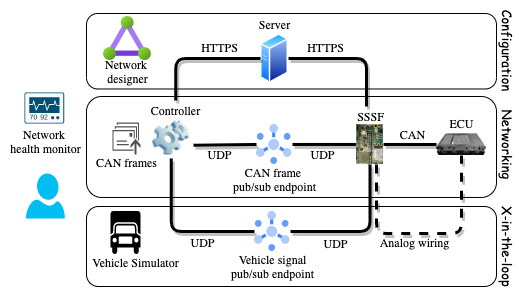
\includegraphics[width=\linewidth]{images/system_design.drawio.png}
    \caption{Proposed System}
    \label{fig:system}
\end{figure*}
Figure \ref{fig:system} shows the proposed system design of CANLay. Based on the goals established in the previous section, we identified three different functional objectives of the system: offline configuration of the network overlay and CAN frame and vehicle signal exchange at runtime. A description of the components and their roles in the system is provided next. Following that, a description of the behavioral aspects of the system is provided. Together, these aspects combine to acomplish the functional objectives of the system.

% ECUs in our system are required to interface with Smart Sensors Simulator (SSSF) devices. These devices act as gateways to the CANLay system. At startup they communicate with a central Server thereby registering themselves. This communication happens over HTTP(s). 

% \subsection{Current Status of Development}

\subsection{Component Descriptions}
\subsubsection{Smart Sensor Simulator and Forwarder (SSSF)}
The Smart Sensor Simulator and Forwarder acts as a gateway enabling the ECU to access and more importantly, to be accessed by, the CANLay system. In an active experiment, it acts as a forwarder between the controller and the ECU through User datagram protocol (UDP) channels and CAN interfaces. SSSFs can forward two types of messages. The first type is sensor messages from the vehicle simulator, but, in accordance with the current design goals, this feature is not used and the analog connection between the SSSF and the ECU is shown in a dashed line figure \ref{fig:system}.  
The second type is CAN data carriers from the ECUs connected to them and from other SSSFs in the current experiment. Through the SSSFs, multiple ECUs can actively communicate with each other to create a rich testing environment.

The SSSF is essentially the smart sensor simulator with additional CAN forwarding capabilities. It is a built on a Teesny 3.6 .... a paragraph describing the SSSF's ability...
talk about SD cards
The real time clock on the SSF is synchronized through the network time protocol (NTP).

\subsubsection{Controller}
The Controller is the user's interface to the CANLay system and enables vehicle simulators to communicate with the CANLay network. The Controller’s user interface is used to assist the user in building their virtual testbed. 
It does so by communicating with the central Server over hypertext transfer protocol secure (HTTPS). 
Once the experiment setup is completed the Controller transitions to acting as a gateway for a graphical vehicle simulator to communicate bi-directionally with the CANLay system. It forwards simulator outputs to the publish/subscribe (pub/sub) endpoint and listens for CAN messages from the same.

Add some implementation details - like python, thread etc.
The real time clock on the Controller is synchronized through the network time protocol (NTP).

\subsubsection{Server}
The Server helps in setting up the publishers and subscribers for an experiment. Each device opens and must maintain a persistent transmission control protocol (TCP) connection with the Server while they participate in the CANLay system. Once the TCP connection is established the devices communicate with the Server through HTTP application programming interfaces (API). The Server can monitor the health of the devices and take actions if a device is malfunctioning or goes offline. This also allows the Server to keep track of free devices and free pub/sub endpoints, so it can validate new experiment requests and allocate the requested devices and endpoints without running into race conditions or double use issues that may arise if each Controller was in charge of allocating its own experiment. Finally, the Server keeps track of ongoing experiments and ensures the proper closure of a experiment in the event a device is experiencing issues.

Add some implementation details - like python, thread etc. Sockets.
The Server accepts HTTP API calls. API calls were chosen because they clearly define the object to invoke and the manner in which to invoke it.

% \subsubsection{Vehicle Simulator}
% In theory, the Vehicle Simulator can be any software that provides the user with the ability to control a vehicle in a digital world. To be compatible with CANLay, the Vehicle Simulator must expose its operating signals in some manner. For the purpose of this paper, we chose the CARLA graphical vehicle simulator \cite{Dosovitskiy17}. 

% Although the Carla project mainly focuses on autonomous driving research it exposes its in-game signals through an easy-to-use python api and pays close attention to the scientific details represented in its simulator. While this is not required, the more realistic and accurate the signals are, the easier it will be to transform them into CAN messages. Furthermore, CARLA is highly configurarble, robust and has been used for purposes similar to ours.

% \subsubsection{User Interface to CAN}
% We forward the recieved CAN frame on a virtual CAN (VCAN) interface that is provided by the user at startup. A user can access these frames via socketCAN \footnote{\url{https://www.kernel.org/doc/html/latest/networking/can.html}} and assosiated tools.

\subsubsection{Publish/Subscribe Endpoints}
UDO is used to connect the publishers and subscribers in the CANLay system. 
% A pub/sub endpoint in the CANLay network is a pub/sub address and port pair. Although the CAN frame and Vehicle signal pub/sub endpoints are shown separately in the above diagram for clarity, they are physically a single endpoint in the network. 
The pub/sub model was chosen because it can easily emulate the broadcast nature CAN in that an ECU is subscribed to all other ECUs on the same CAN bus and all other ECUs on that CAN bus are subscribed to that ECU. 

To find a suitable pub/sub mechanism that closely resembled that of a CAN network we used a few criteria. The first is that the transport mechanism must support some form of message broadcasting which enables a sender to send one message that can be received by many receivers without signficant duplication and delay related overheads. The next requirement is that the transport mechanism must enable the devices to receive messages from one or more devices while having to maintain only one connection. 
% In addition the transport mechanism must not have any implicit congestion control or flow control since none is found in CAN networks. Finally, it's preferable if the communication mechanism transported data as individual messages rather than streams of data.

At this time we have chosen UDP multicasting as a suitable pub/sub mechanism as it does not require a message broker with high performance requirements. We realize that multicasting outside a local network may lead to increased cost for the implementers, but the current goal was to test its usability and make future decisions based on the observed throughout. At this time, we are also exploring other potential pub/sub implementations such as MQTT.


\subsubsection{Network health monitor}
A large drawback of connecting devices over a shared/multipurpose network is the increase of networking delays. When a user creates a virtual test bed using CARLay they are logically forming a virtual network for that experiment, but physically each device is still connected to the same network as before. As a result, communication between devices in a virtual test bed could suffer from network delays that are out of the user’s control. The Network Health Monitor provides the user with useful information about the current status of the network so they can ensure that the current network conditions are not affecting their results. The network information is gathered from the perspective of all devices in a experiment rather than collecting it from just the perspective of the Controller. This provides a more full view of the current state of the network.

\subsection{Behavior Descriptions}

\begin{figure*}[t!]
    \centering
    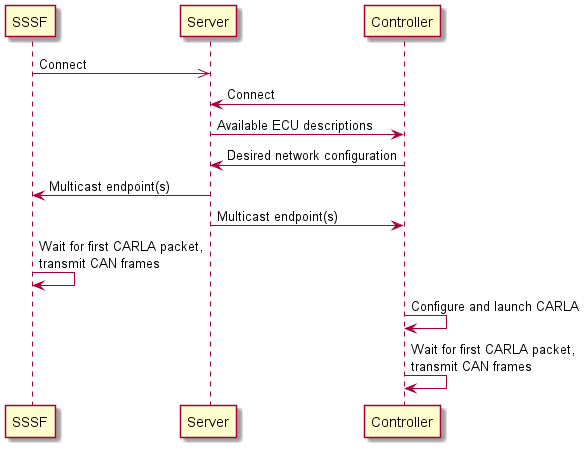
\includegraphics[width=\linewidth]{out/images/connection_setup/connection_setup.png}
    \caption{Setup Activity}
    \label{fig:setup_activity}
\end{figure*}
\subsubsection{Setup (ref. figure \ref{fig:setup_activity})}
While the Server is up and running SSSFs connect to it. SSSFs perform a setup() procedure by reading their inbuit SD card. The type, year, make, model, and serial number of the connected ECUs are required to be included in a predefined file stored on the SD card. 
Next, the SSSF gathers its MAC address and list of attached devices into a JSON and sends it to the Server via a POST to the HTTP API endpoint “\\SSSF\\Register”. 
% The Server will parse and validate the registration. If the registration is satisfactory, it will reply with a code 202 indicating to the SSSF that it has successfully registered with the Server. 
% If the registration data contains invalid data such as a  attached device, or invalid JSON the Server will respond with the appropriate error code and drop the connection. 
If the registration fails, the Server responds with an HTTP 202 error code. Otherwise, the SSSF waits for further instructions from the Server on its TCP/HTTPS port. 

The Controller begins by registering with the Server in a similar manner to the SSSF except that the Controller has no attached devices so it only sends its MAC address to the Server.
% The Server will once again pars/e and validate the registration and respond with the appropriate code. If the Controller successfully registered then it proceeds to make a “GET” to the HTTP API endpoint “\\SSSF”. 
This asked the Server for a list of all of the available SSSF devices. Please note that if a SSSF device is currently being used in another experiment it is not considered available. After the controller has received the list of available devices it presents the available ECUs to the user. Notice that while the Server deals with the SSSF devices a user will typically only be interested in the ECUs that the SSSF is acting as a gateway for. After the user finalizes their selection the Controller sends the selected devices via HTTP POST.

When the Server receives a experiment request it first checks to make sure that the request is coming from a registered Controller. 
Next the Server confirms that the devices are still available. 
If any of the devices are no longer available or become unavailable during the experiment setup process, the Server responds to the Controller with the error code 409 indicating there's a conflict in the selection. 
If the Controller receives this message it starts the experiment selection processes over again. 
If all of the devices are still available the Server then selects an available pub/sub endpoint for the experiment and assigns an index to each device. The index is used in the collection of network statistics which will be explained later on. 
At this time the Server sends the connection data to the controller and selected SSSFs. Connection data contains the unique ID and index of the device, a multicast IP address and port acting as the pub/sub endpoint, and a list containing the ID and attached devices of other nodes in the experiment.

Once endpoints receives the multicast IP addresses they resync with NTP, allocate space for the required data structures, and begin listening for and forwarding messages to and from the pub/sub endpoint. At this point the experiment setup is completed.

% \begin{figure}[t!]
%     \centering
%     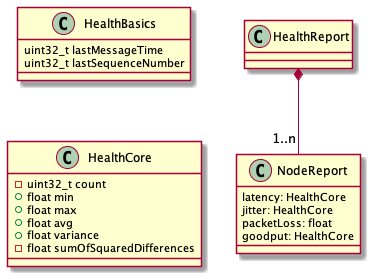
\includegraphics[width=\linewidth]{out/images/network_health/network_health.png}
%     \caption{}
%     \label{fig:}
% \end{figure}
\begin{figure}[t!]
    \centering
    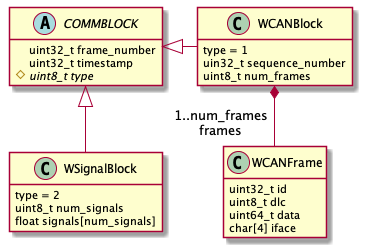
\includegraphics[width=\linewidth]{out/images/data_structures/data_structures.png}
    \caption{Useful Data Structures}
    \label{fig:ds}
\end{figure}
\begin{figure}[t!]
    \centering
    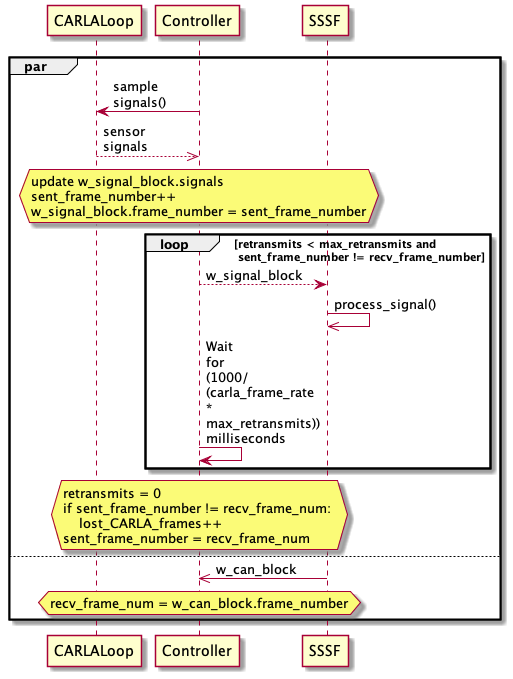
\includegraphics[width=\linewidth]{out/images/signal_control/signal_control.png}
    \caption{Signal Tranmission Activity}
    \label{fig:sig_x}
\end{figure}
\subsubsection{Signal Transmission (ref. \ref{fig:sig_x})} \label{sec:sig_x}

\begin{figure*}[t!]
    \centering
    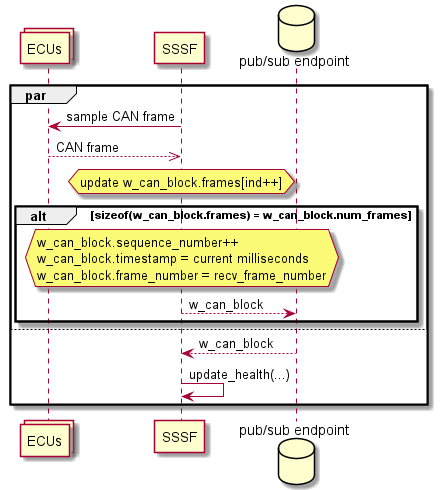
\includegraphics[scale=0.8]{out/images/can_exchange/can_exchange.png}
    \caption{CAN Communication Activity}
    \label{fig:can_x}
\end{figure*}
\subsubsection{CAN Communication (ref. figure \ref{fig:can_x})}
% In order to create the simulated CAN network of ECUs, the devices must be able to communicate with each other with minimum per
% as if they were talking via a CAN bus. 
% Most ECUs do not come with built in ethernet ports and the ability to broadcast CAN frames via Ethernet. So in order to connect an ECU to Ethernet we need a device that can interface with a CAN network and interface with an Ethernet Network. This is why 
% the Smart Sensor Simulator and Forwarder is necessary. It acts as a programmable gateway that can transfer messages between the CAN network and the Ethernet Network.

When the SSSF is in an active experiment it 
% first checks if CAN networks were assigned baud rates. If the CAN network was assigned a baud rate, it 
attempts to read a message from the CAN network. If it reads a message from the CAN network, it proceeds to create the COMMBlock data structure (ref. figure \ref{fig:ds}) that will be written to the CANLay network. In the current scenario we set \texttt{num\_frames} to 1. Therefore, a COMMBlock data structure is transmitted after the receipt of every message.
COMMBlock requires some additional information before it can be written to the network. 
First, a type is added to indicate the subclass it is carrying. In this case the type will be 1, indicating that it is carrying a WCANFrame. 
It also adds the current millisecond timestamp at which it is sending the message
% This is used by other devices to calculate the network latency for the network path from this device. 
, a sequence number that is incremented every time a CAN message is sent
% If other devices on the network detect gaps in the sequence numbers they know that a message has been lost. 
and a frame number of the last frame it received from the Controller.
While the first two are used for network health monitoring (described in section \ref{sec:nethealth}), the last one is used to for retransmission of retranmission of WSignalBlock structures as alread seen in section \ref{sec:sig_x}.
% If it has not received any frames from the Controller then this number will be zero. The last seen frame number indicates to the Controller which SSSFs have and have not received the last sent frame. 
% Also, the SSSF will mark whether this CAN message is a canFD CAN frame. 
The SSSF also marks whether this message requires a response. The CAN message requires a response if its CAN frame’s PGN matches a list received from the user.

After the SSSF is done checking for CAN messages from the CAN network, it moves on to check for messages from the pub/sub network. Again, CAN messages sent to the pub/sub endpoint are considered type 1 messages. So if an SSSF device receives a type 1 message it first checks if the message requires a response. If so, it replies to the pub/sub endpoint with a type 5 message with the frame number equal to the sequence number of the message it just received. Next it updates its network statistics about the device it came from using the sequence number, timestamp, and other metrics from the COMMBlock and then it writes the FlexCAN CAN frame onto its available CAN networks.
% This is supposed to be sudo code btw
    if (msg.type == 1)
    {
        if (msg.needsResponse)
        {
            writeToMcastEndpoint(5. msg.sequenceNumber);
        }
        networkHealth->update(msg);
        if (can0BaudRate) can0.write(msg.canFrame.can);
        if (can1BaudRate) can1.write(msg.canFrame.can);
    }

\subsubsection{Network health monitoring}\label{sec:nethealth}
\begin{figure}[t!]
    \centering
    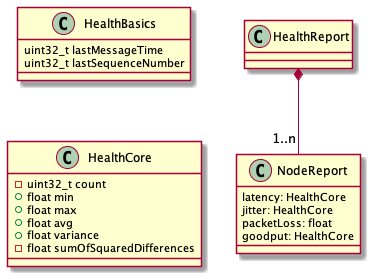
\includegraphics[width=\linewidth]{out/images/network_health/network_health.png}
    \caption{}
    \label{fig:}
\end{figure}
As discussed earlier, monitoring the health of the network is key to ensuring that bad delays or large amounts of packet loss are not affecting your test results. In order to enable the devices to collect network statistics during an active experiment, each message is loaded with additional information. The first piece of additional information is a frame number. The Controller increments the frame number everytime it sends out new signals. When the SSSFs receive a message with a frame number higher than the previous frame number they saw, they send their frame number to the new frame number. Whenever SSSF devices send a message they add that frame number to the top of it. Therefore when a Controller receives a CAN message it can check the last frame the device had received when it sent the CAN message by checking the frame number in the COMMBlock. This system enables acknowledgement of messages without having to send any additional messages. In addition if an SSSF spots a gap in the frame numbers that is larger than 1, then it knows that a frame has been lost.

The type 1 COMMBlock messages (messages containing CAN frames) include a sequence number in addition to the frame number discussed earlier. Whenever an SSSF device sends out a CAN message, it adds a sequence number and increments it by 1. Signals from the controller are sent at the frame rate of the game. This means that with a frame rate of 60fps the Controller is sending messages about 3-4x slower than the message rate seen in on a 250,000 baud ECU operating at nominal bus load. As such we cannot expect the acknowledgement mechanism used for the Controller messages to work for the CAN messages. However other devices can still use the sequence numbers to detect dropped CAN messages by looking for gaps larger than 1.

The next important metric included in the COMMBlock messages is a timestamp. Timestamp is included to allow devices to calculate the latency along the network edge from the sending device to the receiving device. Of course this could be done by performing network tests during an active experiment but unless the latency is guaranteed to always be low, this testing could interrupt the normal flow of the other messages being sent in the experiment. So instead the timestamp is included with each message that is sent so that network health metrics can be calculated on the fly and performed without interrupting the testing. The latency is calculated by subtracting the time at which the message was sent from the time at which the message was received. The downside to this method is that it requires all of the device's clocks to be synchronized as close as possible. With the current basic implementation of the NTP protocol, the devices on average stay within a millisecond or two of each other when they are all referencing an NTP Server on the same network. Unfortunately when the devices use different NTP Servers that are much farther away the devices tend to stray between 5-15 milliseconds from each other. This creates issues when trying to measure the latency of devices that are very close to each other. It's important to note that more advanced implementations of NTP may be able to shrink these numbers.

Overall, these indicators enable each device to calculate four network statistics for every other device on the network namely packet loss, latency, jitter, and goodput. Packet loss is the number of packets determined to be lost along a network edge. Latency is the time it takes for a message to go from the sender to its receiver. Jitter is the variance in latency. There are many different types of network jitter but we use the simplest form which is often called packet jitter or constant jitter which is defined as “packet jitter or packet delay variation (PDV) is the variation in latency as measured in the variability over time of the end-to-end delay across a network” (cite https://networkencyclopedia.com/jitter/). Goodput is the measurement of application level throughput. In our case it is calculated in bytes per second.

Every second the Controller sends out a type 3 message which requests the health report from each device. After each device has sent their health report to the Controller they reset their statistics, keeping only the last message timestamp and the last seen sequence number. This effectively creates a measurement period of 1 second. As the Controller receives the health reports, it updates the network statistic data structure and displays the new results to the user. By collecting health reports from each network node we are able to get the statistics about a network edge from devices on each side of that network edge (how do I explain the importance of the network stats matrix better?).


\section{Usage Example}
\begin{figure*}[t!]
    \centering
    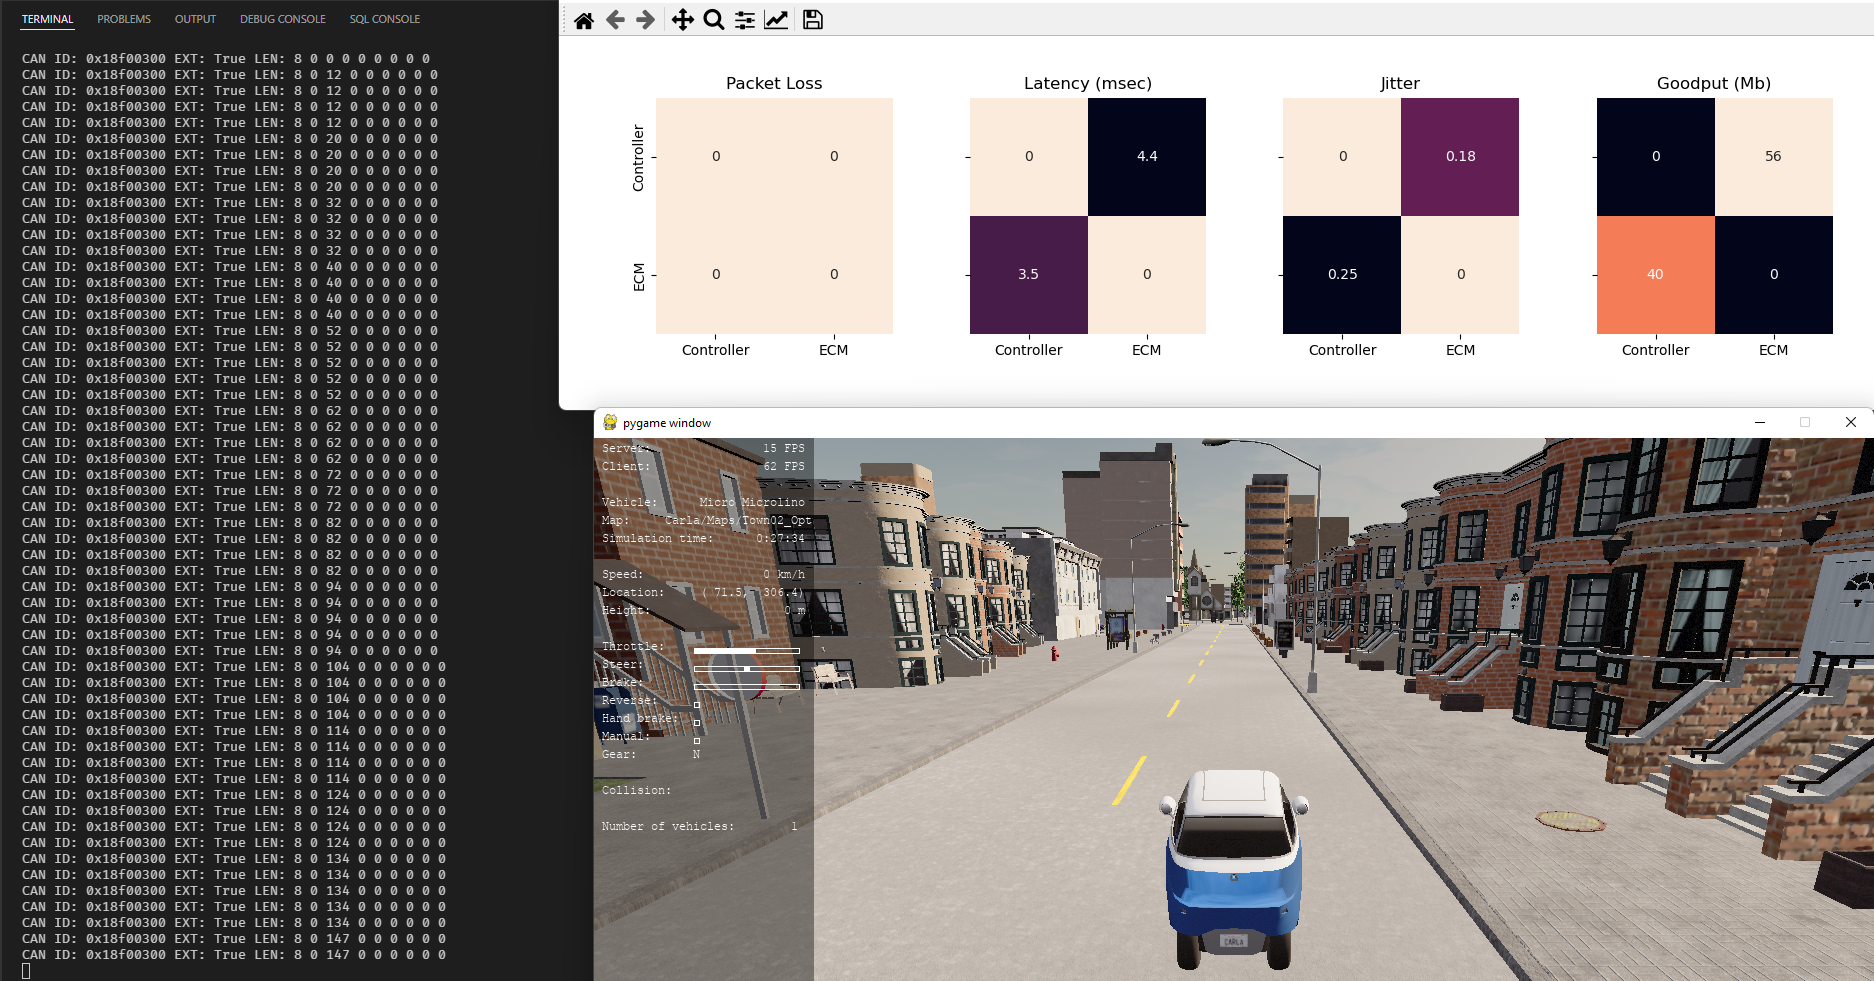
\includegraphics[width=\linewidth]{images/escar_paper_screenshot_all_3 - Copy.png}
    \caption{CANLay at work in the Software Defined Truck}
    \label{fig:usabiity}
\end{figure*}
Figure \ref{fig:usabiity} shows CANLay at work. The windows in the figure display CAN frames on left, the vehicle simulator on the bottom right and CANLay's network health monitoring on the top right. Each of these components were already described in figure \ref{fig:system}. For the current purpose we have been using the CARLA graphical vehicle simulator \cite{Dosovitskiy17}. 
Although the Carla project mainly focuses on autonomous driving research it exposes its in-game signals through an easy-to-use python api and pays close attention to the scientific details represented in its simulator. While this is not required, the more realistic and accurate the signals are, the easier it will be to transform them into CAN messages. In this case, a specific CAN frames is being printed as they are broadcasted on the overlay for this particular experiment. The ID of this frame is defined by the SAE-J1939 standards \cite{society_of_automotive_engineers_sae_nodate} and identifies engine parameters transmitted by an engine control module (ECM). The data bytes carried in the CAN frame are showed next. Of these, the third byte is shown to be changing. This particular byte carries the percentage throttle demanded by the driver. The value is also non-zero on the simulator frontend provided by the CARLA simulator.

On the top right is the network health monitoring window. It shows four matrices showing
four differnet metrics to estimate network health: packet loss, latency in milliseconds, jitter and goodput. The significance of each of these metrics and their calculation methods were already described in the previous section. In this case, the experiment is performed over a gigabit local area network with a layer 3 switch in between an SSSF and a controller. The figure shows no packets were lost while the latency in the last cycle of health report collection was about ~4 milliseconds between the endpoints. Although CANLay does not explicitly perform any latency reducing functions, the general latency of 4 milliseconds is considered to be substainable for seamless CARLA emulation at standard frame rates. In this particular example, the CARLA emulation frame rate was chosen to be 60 frames per second. The jitter is also fairly low in comparsion to the latency. The goodput, i.e. the application data rate is understandibly higher for the controller as it sends WSignalBlock frames that are slightly larger in size than the WCANBlock frames. 

\section{Conclusion and Future Work}
In this paper, we described the concepts behind the design of CANLay, the networking backbone for the Software Defined Truck. SDT is a virtualization based experimentation framework for CAN-based security experiments and CANLay is the carrier of physical control and CAN data over long distance networks. Essentially CANLay enables network virtualization for SDT. CAN is a reliable and low-latency network. CANLay does not explicitly ensure reliability and low latency, but provides a health monitoring service that provides real-time measures of network parameters to the user. This allows the user to make critical decisions about the state of the experiment they are in.

We believe more than one additional works can still be done on CANLay. 
Need response
Dynamic buffer adjustment
 
%-------------------------------------------------------------------------------
\bibliographystyle{plain}
\bibliography{bib}

%%%%%%%%%%%%%%%%%%%%%%%%%%%%%%%%%%%%%%%%%%%%%%%%%%%%%%%%%%%%%%%%%%%%%%%%%%%%%%%%
\end{document}
%%%%%%%%%%%%%%%%%%%%%%%%%%%%%%%%%%%%%%%%%%%%%%%%%%%%%%%%%%%%%%%%%%%%%%%%
